\documentclass[[12pt,twoside]{book}
\usepackage{_my_document_style}
\begin{document}
%
\def\mySweepLEWingDEG{0.000000}
\def\mySweepLEWingRAD{0.000000}
\def\myChordRootWingMT{2.500000}
\def\myChordTipWingMT{1.000000}
\def\mySpanWingMT{16.000000}
\def\myTaperRatioWing{0.400000}
\def\myAreaWingMTsquared{28.000000}
\def\myAspectRatioWing{9.142857}
\def\myMach{0.400000}
\def\myCLAlphaRootWingRAD{6.150000}
\def\myCLAlphaRootWingDEG{0.107338}
\def\myCLAlphaTipWingRAD{6.050000}
\def\myCLAlphaTipWingDEG{0.105592}
\def\myAlphaZeroLiftRootWingDEG{-3.000000}
\def\myAlphaZeroLiftTipWingDEG{-1.500000}
\def\myAlphaZeroLiftRootWingRAD{-0.052360}
\def\myAlphaZeroLiftTipWingRAD{-0.026180}
\def\myXsiacRootWing{0.250000}
\def\myXsiacTipWing{0.250000}
\def\myCmZeroRootWing{-0.080000}
\def\myCmZeroTipWing{-0.100000}
\def\mySweepQuarterChordWingDEG{-3.297150}
\def\mySweepQuarterChordWingRAD{-0.057546}
\def\myMACWingMT{1.857143}
\def\myYMACWingMT{3.428571}
\def\myXMACLEToApexWingMT{0.000000}
\def\myKOneACDatcomWing{1.342000}
\def\myKTwoACDatcomWing{0.000000}
\def\myXACOverChordRootDatcomWing{0.176000}
\def\myXsiACWing{0.236192}
\def\myACWingToApexWingMT{0.438642}
\def\myACWingToMACLEWingMT{0.438642}
\def\myCoeffAChordWing{-0.187500}
\def\myCoeffBChordWingMT{2.500000}
\def\myCoeffAAeroTwistWingRADMT{0.003272}
\def\myCoeffACmZeroWingMT{-0.002500}
\def\myCoeffBCmZeroWing{-0.080000}
\def\myCmZeroAWing{-0.087308}
\def\myCmZeroBWing{-0.003465}
\def\myCmZeroWing{-0.090772}
\def\myCoeffAWing{-0.500000}
\def\myCoeffBWing{0.059375}
\def\myCoeffCWing{-0.000469}
\def\myCoeffDWing{-0.000088}
\def\myCoeffEWing{-0.043792}
\def\myCoeffFWing{0.027072}
\def\myCoeffGWing{-0.004997}
\def\myCoeffHWing{0.000241}
\def\myCoeffIWing{0.230009}
\def\myCoeffJWing{-0.084804}
\def\myCoeffKWing{0.005203}
\def\myCoeffLWing{-0.000010}
\def\myCLAlphaMeanWingRAD{6.107143}
\def\myCoeffAClalphaWingRADMT{-0.012500}
\def\myCoeffBClalphaWingRAD{6.150000}
\def\myTwistWingDEG{-2.500000}
\def\myTwistWingRAD{-0.043633}
\def\myCoeffATwistWingRADMT{-0.005454}
\def\myCoeffBAeroTwistWingRAD{-0.052360}
\def\myAlphaZeroLiftWingRAD{-0.022440}
\def\myAlphaZeroLiftWingDEG{-1.285714}

%
%
\begin{myExampleX}{Pitching moment around the wing aerodynamic center}{\ding{46}}% \ \Keyboard\ %
\label{example:Wing:Cmac:A}
%
\noindent
Consider the straight-edged wing shown in the figure~\ref{fig:Wing:Cmac:Results:A}
whose sweep angle of the leading edge is null,
that is $\Lambda_\mathrm{le}=\SI[round-precision=0]{\mySweepLEWingDEG}{\deg}$.
The remaining characteristics of the wing are as follows:

\smallskip
\noindent
\adjustbox{left=\textwidth}{%
  \adjustbox{right=0.39\textwidth}{%
    \emph{chords}:
  }\rule{0.5em}{0pt}% --> SPACER
  \adjustbox{left=0.59\textwidth}{%
    $c_\mathrm{r}=\SI[round-precision=2]{\myChordRootWingMT}{\metre}$,
    $c_\mathrm{t}=\SI[round-precision=0]{\myChordTipWingMT}{\metre}$,
    $\lambda = \SI[round-precision=2]{\myTaperRatioWing}{}$,
  }%
}

\smallskip
\noindent
\adjustbox{left=\textwidth}{%
  \adjustbox{right=0.39\textwidth}{%
    \emph{wingspan and surface}:
  }\rule{0.5em}{0pt}% --> SPACER
  \adjustbox{left=0.59\textwidth}{%
    $b=\SI[round-precision=0]{\mySpanWingMT}{\metre}$,
    $S=\SI[round-precision=0]{\myAreaWingMTsquared}{\meter^2}$,
    $\AR = \SI[round-precision=2]{\myAspectRatioWing}{}$,
  }%
}

\smallskip
\noindent
\adjustbox{left=\textwidth}{%
  \adjustbox{right=0.39\textwidth}{%
    \emph{gradient $C_{\ell_\mathlarger{\alpha}}$ of profile}:
  }\rule{0.5em}{0pt}% --> SPACER
  \adjustbox{left=0.59\textwidth,minipage=[t]{0.59\textwidth}}{%
    $C_{\ell_\mathlarger{\alpha},\mathrm{r}}=\SI[round-precision=2]{\myCLAlphaRootWingRAD}{\radian^{-1}}=\SI[round-precision=4]{\myCLAlphaRootWingDEG}{\deg^{-1}}$,
    \\
    $C_{\ell_\mathlarger{\alpha},\mathrm{t}}=\SI[round-precision=2]{\myCLAlphaTipWingRAD}{\radian^{-1}}=\SI[round-precision=4]{\myCLAlphaTipWingDEG}{\deg^{-1}}$,
  }%
}

\smallskip
\noindent
\adjustbox{left=\textwidth}{%
  \adjustbox{right=0.39\textwidth}{%
    \emph{zero lift angles}:
  }\rule{0.5em}{0pt}% --> SPACER
  \adjustbox{left=0.59\textwidth,minipage=[t]{0.59\textwidth}}{%
    $\alpha_{0\ell,\mathrm{r}}=\SI[round-precision=3]{\myAlphaZeroLiftRootWingRAD}{\radian}
      =\SI[round-precision=1]{\myAlphaZeroLiftRootWingDEG}{\deg}$,\\
    $\alpha_{0\ell,\mathrm{t}}=\SI[round-precision=3]{\myAlphaZeroLiftTipWingRAD}{\radian}
      =\SI[round-precision=1]{\myAlphaZeroLiftTipWingDEG}{\deg}$,
  }%
}

\smallskip
\noindent
\adjustbox{left=\textwidth}{%
  \adjustbox{right=0.39\textwidth}{%
    \emph{aerodynamic profile centers}:
  }\rule{0.5em}{0pt}% --> SPACER
  \adjustbox{left=0.59\textwidth}{%
    $\bar{x}_{\mathrm{ac,2D},\mathrm{r}}=\SI[round-precision=2]{\myXsiacRootWing}{}$,
    $\bar{x}_{\mathrm{ac,2D},\mathrm{t}}=\SI[round-precision=2]{\myXsiacTipWing}{}$,
  }%
}

\smallskip
\noindent
\adjustbox{left=\textwidth}{%
  \adjustbox{right=0.39\textwidth}{%
    \emph{coefficients $C_{m_\mathlarger{\mathrm{ac}}}$ of profile}:
  }\rule{0.5em}{0pt}% --> SPACER
  \adjustbox{left=0.59\textwidth}{%
    $C_{m_\mathlarger{\mathrm{ac}},\mathrm{r}}=\SI[round-precision=3]{\myCmZeroRootWing}{}$,
    $C_{m_\mathlarger{\mathrm{ac}},\mathrm{t}}=\SI[round-precision=3]{\myCmZeroTipWing}{}$,
  }%
}

\smallskip
\noindent
\adjustbox{left=\textwidth}{%
  \adjustbox{right=0.39\textwidth}{%
    \emph{flight condition}:
  }\rule{0.5em}{0pt}% --> SPACER
  \adjustbox{left=0.59\textwidth}{%
    $\Mach = \SI[round-precision=2]{\myMach}{}$.
  }%
}

\smallskip
For the assigned wing we want to calculate the coefficient \smash{$C_{\mathcal{M}_\mathlarger{\mathrm{ac}}}$}.

\medskip
The sweep angle of the quarter-chord line --- line that coincides in this case with the line of aerodynamic centers of the wing sections --- it is calculated as follows:
\[
\begin{split}
\tan
\Lambda_{c/4}
   = \tan\Lambda_\mathrm{le}-\dfrac{(4/4)(1-\lambda)}{\AR(1+\lambda)}
   & {}=
    \tan (\SI[round-precision=0]{\mySweepLEWingRAD}{\radian})
      - \dfrac{
         \num[round-precision=2]{1.0}
         \cdot (1-\SI[round-precision=2]{\myTaperRatioWing}{})
      }{
         \num[round-precision=2]{\myAspectRatioWing}
         \cdot (1+\SI[round-precision=2]{\myTaperRatioWing}{})} 
\\[3pt]
   & \Rightarrow
   \quad
   \Lambda_{c/4}
      = \mathunderline{mydarkblue}{ \SI[round-precision=4]{\mySweepQuarterChordWingRAD}{\radian} }
      = \mathunderline{mydarkblue}{ \SI[round-precision=1]{\mySweepQuarterChordWingDEG}{\deg} }
\end{split}
\]
The assigned wing, therefore, has a small and negative sweep angle $\Lambda_{c/4}$.

The mean aerodynamic chord is in this case
\[
\bar{c} = \frac{2}{3} \, c_\mathrm{r} \, \frac{1+\lambda + \lambda^2}{1+\lambda}
  =
    \num{0.667} \cdot \SI[round-precision=2]{\myChordRootWingMT}{\metre}
      \cdot 
        \frac{
          1 + \SI[round-precision=2]{\myTaperRatioWing}{} + \SI[round-precision=2]{\myTaperRatioWing}{}^2
        }{
          1 + \SI[round-precision=2]{\myTaperRatioWing}{}
        }
    = \mathunderline{mydarkblue}{ \SI[round-precision=2]{\myMACWingMT}{\metre} }
\]

The longitudinal distance of the leading edge of the mean aerodynamic chord from the
leading edge of the root chord is null,
$X_{\mathrm{le},\bar{c}} = \SI[round-precision=0]{\myXMACLEToApexWingMT}{\metre}$, 
being $\Lambda_\mathrm{le}$ null.

The station $Y_{\bar{c}}$ to which the law of the chords $c(Y)$ assumes value$\bar{c}$ is
\[
Y_{\bar{c}} 
  =
    \frac{b}{6} \, \frac{1+2\lambda}{1+\lambda}
  =
    \frac{\SI[round-precision=0]{\mySpanWingMT}{\metre}}{6}
      \cdot 
      \frac{
        1 + 2\cdot\SI[round-precision=2]{\myTaperRatioWing}{}
      }{
        1 + \SI[round-precision=2]{\myTaperRatioWing}{}
      }
    = \mathunderline{mydarkblue}{ \SI[round-precision=2]{\myYMACWingMT}{\metre} }
\]


For the assigned flight Mach number
the aerodynamic center of the wing is calculated as in the example~\ref{example:Wing:Aerodynamic:Center:Of:A:Finite:Wing}.
From the data and the figure~\ref{fig:Wing:Ac:K:One:Plots}
we get
\[
\lambda=\SI[round-precision=2]{\myTaperRatioWing}{}
%
%\quad \Longrightarrow \quad
%\quad \begin{array}{@{}c@{}} \myIconGraph \\[-4pt] \Longrightarrow \end{array} \quad
\adjustbox{center=4em}{%
  \adjustbox{lap=\width}{\raisebox{2.2ex}[0pt][0pt]{\myIconGraph}}$\Longrightarrow$%
}
%
K_1
  = \mathunderline{mydarkblue}{ \SI[round-precision=3]{\myKOneACDatcomWing}{} }
\]
from the figure~\ref{fig:Wing:Ac:K:Two:Plots}
we can obtain
\[
\Lambda_\mathrm{le} = \SI[round-precision=0]{\mySweepLEWingDEG}{\deg}\;,\;\,
\AR = \SI[round-precision=1]{\myAspectRatioWing}{}\;,\;\,
\lambda=\SI[round-precision=2]{\myTaperRatioWing}{}
%\quad \Longrightarrow \quad
%\quad \begin{array}{@{}c@{}} \myIconGraph \\[-4pt] \Longrightarrow \end{array} \quad
\adjustbox{center=4em}{%
  \adjustbox{lap=\width}{\raisebox{2.2ex}[0pt][0pt]{\myIconGraph}}$\Longrightarrow$%
}
%
K_2 
  = \mathunderline{mydarkblue}{ \SI[round-precision=0]{\myKTwoACDatcomWing}{} }
\]
from the figure~\ref{fig:Wing:Ac:X:AC:From:Apex:Plots}
we get
\[
\Lambda_\mathrm{le} = \SI[round-precision=0]{\mySweepLEWingDEG}{\deg}\;,\;\,
\Mach = \SI[round-precision=2]{\myMach}{}\;,\;\,
\AR = \SI[round-precision=1]{\myAspectRatioWing}{}\;,\;\,
\lambda=\SI[round-precision=2]{\myTaperRatioWing}{}
%
%\quad \Longrightarrow \quad
%\quad \begin{array}{@{}c@{}} \myIconGraph \\[-4pt] \Longrightarrow \end{array} \quad
\adjustbox{center=4em}{%
  \adjustbox{lap=\width}{\raisebox{2.2ex}[0pt][0pt]{\myIconGraph}}$\Longrightarrow$%
}
%
\frac{X'_{\mathrm{ac}}}{c_\mathrm{r}}
  = \mathunderline{mydarkblue}{ \SI[round-precision=3]{\myXACOverChordRootDatcomWing}{} }
\]
%
It is thus obtained
\[
\frac{x_{\mathrm{ac}}}{\bar{c}} 
  = K_1 \left( \frac{X'_{\mathrm{ac}}}{c_\mathrm{r}} - K_2  \right)
  = \SI[round-precision=3]{\myKOneACDatcomWing}{} \,
    \Big(  
      \SI[round-precision=3]{\myXACOverChordRootDatcomWing}{} 
        - \SI[round-precision=0]{\myKTwoACDatcomWing}{}  
    \Big)
  = \mathunderline{mydarkblue}{ \SI[round-precision=3]{\myXsiACWing}{} } 
\]
%
Therefore, the location $X_\mathrm{ac}$ can be calculated as

\[
X_\mathrm{ac} 
  =
    X_{\mathrm{le},\bar{c}} + \left( \frac{x_{\mathrm{ac}}}{\bar{c}} \right) \bar{c}
=
    \SI[round-precision=0]{\myXMACLEToApexWingMT}{\metre}
      + \SI[round-precision=3]{\myXsiACWing}{}
        \cdot \SI[round-precision=2]{\myMACWingMT}{\metre}
      = \SI[round-precision=0]{\myXMACLEToApexWingMT}{\metre}
        % + \calcSI[round-precision=2,fixed-exponent=0,scientific-notation=fixed]{\myXsiACWing*\myMACWingMT}{\metre}
        + \SI[round-precision=2]{\myACWingToMACLEWingMT}{\metre} 
    = \mathunderline{mydarkblue}{ 
      %\calcSI[round-precision=2,fixed-exponent=0,scientific-notation=fixed]{
      %  \myXMACLEToApexWingMT + \myXsiACWing*\myMACWingMT
      %}{\metre} 
      \SI[round-precision=2]{\myACWingToApexWingMT}{\metre} 
    }%
\]

The position of the wing aerodynamic center identifies a line normal to the center plane
equation $X=X_\mathrm{ac}$ against which the law of arms can be calculated
of the basic load
\[
x_\mathrm{b}(Y) 
  = X_\mathrm{ac} 
    - \Big[ Y \tan \Lambda_\mathrm{le} + \bar{x}_{\mathrm{ac,2D}} (Y) \, c(Y) \Big]
\]
The function $\bar{x}_{\mathrm{ac,2D}}(Y)$ represents the dimensionless distance from the aerodynamic profile center
at the station $Y$ rom the leading edge of the local chord. 
For the assigned wing this function coincides with the constant law
$\bar{x}_{\mathrm{ac,2D}}(Y) = \frac{1}{4}$ and the previous expression,
being $\Lambda_\mathrm{le}$ null, in our case it becomes
\[
x_\mathrm{b}(Y) = X_\mathrm{ac} - \frac{1}{4} \, c(Y)
\]

The pitching moment coefficient $C_{\mathcal{M}_\mathlarger{\mathrm{ac}}}$ of the wing
around its aerodynamic center is given by the formula
\[
C_{\mathcal{M}_\mathlarger{\mathrm{ac}}}
  = 
    \underbrace{% needs mt2pro, \underbrace otherwise
      %
      \frac{2}{S\,\bar{c}} \int_0^{b/2} C_{m_\mathlarger{\mathrm{ac}},\mathrm{2D}}(Y) \; c^2(Y)\, \diff{Y}
      %
      %\rule[-1.2em]{0pt}{2em}% --> SPACER
    }_{ \mathlarger{ C_{\mathcal{M}_\mathlarger{\mathrm{ac,a}}} } } 
    +
    \underbrace{% needs mt2pro, \underbrace otherwise
      %
      \frac{2}{S\,\bar{c}} \int_0^{b/2} \big(cC_{\ell}\big)_\mathrm{b}(Y) \; x_\mathrm{b}(Y)\, \diff{Y}
      %
      %\rule[-1.2em]{0pt}{2em}% --> SPACER
    }_{ \mathlarger{ C_{\mathcal{M}_\mathlarger{\mathrm{ac,b}}} } } 
\]
%
where 
\begin{compactenum}[{\color{gray}$\bullet$}]%[(\itshape i\upshape)]
\item
$C_{m_\mathlarger{\mathrm{ac}},\mathrm{2D}}(Y)$ is the law of the coefficients of
moment of the profiles around the aerodynamic center of section,
\item
$\big(cC_{\ell}\big)_\mathrm{b}(Y) = c(Y) \, C_{\ell,\mathrm{b}} (Y)$ it is the product of the local chord
$c(Y)$ and the lift coefficient \emph{basic} of section
$C_{\ell,\mathrm{b}}(Y)$ --- present when
the wing is placed at the zero lift angle $\alpha_{0L}$ (angle measured with respect to the root chord),
\item
$x_\mathrm{b}(Y)$ is the arm between the point of application of the local basic load and the center
aerodynamic wing.
\end{compactenum}

The above formula shows that the coefficient \smash{$C_{\mathcal{M}_\mathlarger{\mathrm{ac}}}$}
is the sum of the two contributions:
\begin{compactenum}[\itshape a\normalfont)]
\item
$C_{\mathcal{M}_\mathlarger{\mathrm{ac,a}}}$, obtainable by accumulating the pure couples 
  \[
    \diff{}\mathcal{M}_{\mathrm{ac},\mathrm{a}} 
      = C_{m_\mathlarger{\mathrm{ac}},\mathrm{2D}}(Y) \; \bar{q}_\infty \,
        \underbrace{% needs mt2pro, \underbrace otherwise
          c(Y)\diff{Y}
        }_{ \mathlarger{ \diff{S} } }
          \, c(Y)
    = \bar{q}_\infty \, C_{m_\mathlarger{\mathrm{ac}},\mathrm{2D}}(Y) \, c^2(Y) \, \diff{Y} 
  \]
\item
$C_{\mathcal{M}_\mathlarger{\mathrm{ac,b}}}$,obtainable by accumulating the transport moments
  \[
    \diff{}\mathcal{M}_{\mathrm{ac},\mathrm{b}} 
      = C_{\ell,\mathrm{b}}(Y)\,x_\mathrm{b}(Y)\; \bar{q}_\infty \, 
        \underbrace{% needs mt2pro, \underbrace otherwise
          c(Y)\diff{Y}
        }_{ \mathlarger{ \diff{S} } }
    = \bar{q}_\infty \, \big( cC_{\ell} \big)_\mathrm{b} (Y) \,x_\mathrm{b}(Y)\, \diff{Y}
  \]
\hfill(note that the arm $x_b$ has the dimensions of a length)
\end{compactenum}

\noindent
These contributions are integrated along the wingspan and dimensionless by dividing them
per $\bar{q}_\infty S \bar{c}$.

As for the term $C_{\mathcal{M}_\mathlarger{\mathrm{ac,a}}}$,
proceeding as shown in the example~\ref{example:Zero:Lift:Angle:Of:A:Finite:Wing}
it is obtained
\[
c \big( Y \big) = A_c \, Y + B_c
  = \SI[round-precision=3]{\myCoeffAChordWing}{} \, Y
    + \SI[round-precision=2]{\myCoeffBChordWingMT}{\metre}
\]
and, similarly, it arises
\[
C_{m_\mathlarger{\mathrm{ac}}} \big( Y \big) 
  = A_{C_{m_\mathlarger{\mathrm{ac}}}} \, Y + B_{C_{m_\mathlarger{\mathrm{ac}}}}
\]
with
\[
A_{C_{m_\mathlarger{\mathrm{ac}}}}
  = \frac{C_{m_\mathlarger{\mathrm{ac}},\mathrm{t}} 
    - C_{m_\mathlarger{\mathrm{ac}},\mathrm{r}}}{b/2}
  = 
    2 \frac{
      \SI[round-precision=3]{\myCmZeroTipWing}{} 
      - ( \SI[round-precision=3]{\myCmZeroRootWing}{} )
    }{
      \SI[round-precision=2]{\mySpanWingMT}{\metre}
    }
  = 
    \mathunderline{mydarkblue}{ 
      \SI[round-precision=5]{\myCoeffACmZeroWingMT}{\metre^{-1}} 
    }
\]
\[
B_{C_{m_\mathlarger{\mathrm{ac}}}}
  = C_{m_\mathlarger{\mathrm{ac}},\mathrm{r}}
  = \mathunderline{mydarkblue}{ \SI[round-precision=3]{\myCoeffBCmZeroWing}{} }
\]
i.e.
\[
C_{m_\mathlarger{\mathrm{ac,2D}}} \big( Y \big) 
  = A_{C_{m_\mathlarger{\mathrm{ac}}}} \, Y + B_{C_{m_\mathlarger{\mathrm{ac}}}}
  = \SI[round-precision=5]{\myCoeffACmZeroWingMT}{\metre^{-1}} \, Y
    % +
    \SI[round-precision=3]{\myCoeffBCmZeroWing}{}
\]
%
Therefore, the formula for calculating the contribution due to pure couples provides
\[
\begin{split}
C_{\mathcal{M}_\mathlarger{\mathrm{ac,a}}}
  & {}= \frac{2}{S\,\bar{c}} \int_0^{b/2} 
    C_{m_\mathlarger{\mathrm{ac}},\mathrm{2D}}(Y) \; c^2(Y)\, \diff{Y}
\\
  & {}= 
  \frac{2}{S\,\bar{c}} \int_0^{b/2} 
    \Big( 
      A_{C_{m_\mathlarger{\mathrm{ac}}}} \, Y + B_{C_{m_\mathlarger{\mathrm{ac}}}} 
    \Big)
    \Big( A_c \, Y + B_c \Big)^{\! 2}
    \, \diff{Y}
\\
  & {}= 
  \frac{2}{S\,\bar{c}} \int_0^{b/2} 
    \Big( 
      \SI[round-mode=figures,round-precision=3,
        fixed-exponent=0,scientific-notation=fixed]{\myCoeffAWing}{\metre^2}
      + 
      \SI[round-mode=figures,round-precision=3,
        %fixed-exponent=2,
        %scientific-notation=fixed
        ]{\myCoeffBWing}{\metre}\, Y
      \SI[round-mode=figures,round-precision=3,
        fixed-exponent=-4,
        scientific-notation=fixed % engineering % 
        ]{\myCoeffCWing}{}\, Y^2
      \SI[round-mode=figures,round-precision=3,
        fixed-exponent=-4,
        scientific-notation=fixed
        ]{\myCoeffDWing}{\metre^{-1}}\, Y^3
    \Big)
    \, \diff{Y}
\\
  & {}= \mathunderline{mydarkblue}{ \SI[round-precision=4]{\myCmZeroAWing}{} }
\end{split}
\]
Observe that the value of the definite integral can be obtained by developing symbolically
the integrand function which is a degree polynomial $3$ in the variable $Y$.

\smallskip
From the aerodynamics it is known that for a generic angle of attack $\alpha$ to which the wing produces a lift
coefficient $C_L$,
the $\gamma$\emph{wing span loading} can be expressed as
\[
\gamma(Y) \triangleq \frac{c(Y) \, C_\ell (Y)}{2 b} = C_L \, \gamma_{\mathrm{a}1}(Y) + \gamma_\mathrm{b}(Y) 
\]
Wing loading is the sum of the  \emph{additional} loading $C_L \, \gamma_{\mathrm{a}1}(Y)$
--- a contribution that vanishes at the zero lift angle, in which $C_L=0$ ---
and of the \emph{basic} loading $\gamma_\mathrm{b}(Y)$.
The latter, in particular, is trivially null for non-twisted wings (neither geometrically nor aerodynamically)
and, in general, it has a variation law with the $Y$ whose diagram subtends a null area:
\[
\int_0^{1} \gamma_\mathrm{b}(\eta) \diff{\eta} = 0 \qquad \text{con $\eta \triangleq \dfrac{Y}{b/2}$}
\]

In the calculation formula of \smash{$C_{\mathcal{M}_\mathlarger{\mathrm{ac}},b}$}
compare $\big(cC_{\ell}\big)_\mathrm{b}(Y) = 2b\gamma_\mathrm{b}(Y)$.
This loading law can be determined numerically or in an approximate way
from the knowledge of the laws of geometric warping $\epsilon_\mathrm{g}(Y)$ and aerodynamic
$\alpha_{0\ell}(Y)$and the zero lift angle of the wing $\alpha_{0L}$.

The approximate expression of the basic loading, known from the Vortex Theory of Finite Wings, is the following:
\[
\big(cC_{\ell}\big)_\mathrm{b}(Y)
  = \frac{1}{2} \, c(Y) \, C_{\ell_\mathlarger{\alpha}}(Y) \,
    \bigg\{ \alpha_{0L} - \Big[ \alpha_{0\ell}\big(Y\big) - \epsilon_\mathrm{g}\big(Y\big) \Big] \bigg\}
\]
in which the factor $\frac{1}{2}$ consider the three-dimensional effects in the surrounding region
at the center line of the wing.
%
In the previous formula we must find the expression of the law of lift gradients.
As a first approximation it can be posed
$C_{\ell_\mathlarger{\alpha}} (Y)=2\pi$; alternatively we obtain the following linear law:
\smash{$C_{\ell_\mathlarger{\alpha}} \big( Y \big) = A_{C_{\ell_\alpha}} \, Y + B_{C_{\ell_\alpha}}$}.

Proceeding as shown in the example~\ref{example:Zero:Lift:Angle:Of:A:Finite:Wing}
is obtained
%\[
%c \big( Y \big) = A_c \, Y + B_c
%  = \SI[round-precision=3]{\myCoeffAChordWing}{} \, Y
%    + \SI[round-precision=2]{\myCoeffBChordWingMT}{\metre}
%\]

\[
\alpha_{0\ell} \big( Y \big) = A_{\alpha} \, Y + B_{\alpha}
  = (\SI[round-precision=5]{\myCoeffAAeroTwistWingRADMT}{\radian/\metre}) \, Y
    \SI[round-precision=4]{\myAlphaZeroLiftRootWingRAD}{\radian}
\]

\[
\epsilon_\mathrm{g} \big( Y \big) = A_{\epsilon} \, Y + B_{\epsilon}
  = (\SI[round-precision=5]{\myCoeffATwistWingRADMT}{\radian/\metre}) \, Y
\]

\noindent
and
\[
C_{\ell_\mathlarger{\alpha}} \big( Y \big) = A_{C_{\ell_\alpha}} \, Y + B_{C_{\ell_\alpha}}
  = \SI[round-precision=5]{\myCoeffAClalphaWingRADMT}{\big(\radian\,\metre\big)^{-1}} \, Y
    + \SI[round-precision=3]{\myCoeffBClalphaWingRAD}{\radian^{-1}}
\]

It is also obtained
\[
\begin{split}
\alpha_{0L} 
  & {}= \frac{2}{S} \int_0^{b/2} 
    \Big[ 
      \alpha_{0\ell}\big(Y\big) - \epsilon_\mathrm{g}\big(Y\big) 
    \Big] \, c(Y) \diff{Y}
\\[3pt]
  & {}= \frac{2}{S} \int_0^{b/2} 
    \bigg[ \Big( A_{\alpha} \, Y + B_{\alpha} \Big) - A_{\epsilon} \, Y \bigg] \Big( A_c Y + B_c \Big)
      \diff{Y}
  = \mathunderline{mydarkblue}{ \SI[round-precision=4]{\myAlphaZeroLiftWingRAD}{\radian} }
  = \mathunderline{mydarkblue}{ \SI[round-precision=1]{\myAlphaZeroLiftWingDEG}{\deg} }
\end{split}
\]

The calculation formula of \smash{$C_{\mathcal{M}_\mathlarger{\mathrm{ac}},b}$} thus becomes
\[
\begin{split}
C_{\mathcal{M}_\mathlarger{\mathrm{ac,b}}} 
  & {}=
  \frac{2}{S\,\bar{c}} \int_0^{b/2} \big(cC_{\ell}\big)_\mathrm{b}(Y) \; x_\mathrm{b}(Y)\, \diff{Y}
\\[1pt]
  & {}=
  \frac{1}{S\,\bar{c}} \int_0^{b/2} \;\;
% \big(cC_{\ell}\big)_\mathrm{b}(Y)
%\cancel{2}\;
\overbrace{% needs mtp2pro
%\frac{1}{\cancel{2}}
\rule{0pt}{2em}
c(Y) \, C_{\ell_\mathlarger{\alpha}}(Y) \,
    \bigg\{ \alpha_{0L} - \Big[ \alpha_{0\ell}\big(Y\big) - \epsilon_\mathrm{g}\big(Y\big) \Big] \bigg\}
}^{ \mathlarger{ \big(cC_{\ell}\big)_\mathrm{b}(Y) } }
\\[3pt]
  & \rule{4cm}{0pt}
%
% x_\mathrm{b}(Y) 
    \cdot
    \underbrace{% needs mtp2pro
    \bigg\{ 
      X_\mathrm{ac} 
        - \Big[ Y \tan \Lambda_\mathrm{le} + \bar{x}_{\mathrm{ac,2D}} (Y) \, c(Y) \Big]
    \bigg\} 
    }_{ \mathlarger{ x_\mathrm{b}(Y) } }
    \, \diff{Y}
\end{split}
\]
\noindent
Replacing the previously found values is obtained
\[
 \begin{split}
C_{\mathcal{M}_\mathlarger{\mathrm{ac,b}}} 
  & {}=
  \frac{1}{S\,\bar{c}} \int_0^{b/2}
    %\overcbrace{% needs mtp2pro
    % c(Y) 
    \Big( A_c Y + B_c \Big)
    \, 
    \overbrace^{ \mathlarger{ \big(cC_{\ell}\big)_\mathrm{b}(Y) } }
\\[2pt]
  & \hfill \rule{6cm}{0pt}
%
% x_\mathrm{b}(Y)
    \cdot
    %\undercbrace_{ \mathlarger{ x_\mathrm{b}(Y) } }
    \, \diff{Y}
\\[2pt]
  & {}= 
  \frac{2}{S\,\bar{c}} \int_0^{b/2} 
    \Big( 
      \SI[round-mode=figures,round-precision=3,
        %fixed-exponent=0,
        %scientific-notation=fixed
        ]{\myCoeffEWing}{\metre^2}
      + 
      \SI[round-mode=figures,round-precision=3,
        %fixed-exponent=2,
        %scientific-notation=fixed
        ]{\myCoeffFWing}{\metre}\, Y
      \SI[round-mode=figures,round-precision=3,
        fixed-exponent=-4,
        scientific-notation=fixed % engineering % 
        ]{\myCoeffGWing}{}\, Y^2
      +
      \SI[round-mode=figures,round-precision=2,
        fixed-exponent=-4,
        scientific-notation=fixed
        ]{\myCoeffHWing}{\metre^{-1}}\, Y^3
    \Big)
    \, \diff{Y}
\\[4pt]
  & {}= \mathunderline{mydarkblue}{ \SI[round-precision=5]{\myCmZeroBWing}{} }
\end{split}
\]
Observe that the value of the definite integral can be obtained by developing symbolically
the integrand function which is a degree polynomial $3$ (in this particular case) in the variable $Y$.

Finally, the value of the wing's pitch moment coefficient around its aerodynamic center
is
\[
C_{\mathcal{M}_\mathlarger{\mathrm{ac}}} 
  = C_{\mathcal{M}_\mathlarger{\mathrm{ac,a}}} + C_{\mathcal{M}_\mathlarger{\mathrm{ac,b}}}
  = \SI[round-precision=4]{\myCmZeroAWing}{} 
    +
    ( \SI[round-precision=5]{\myCmZeroBWing}{} )
  = \mathunderline{mydarkblue}{ \SI[round-precision=4]{\myCmZeroWing}{} }
\]

In the figure~\ref{fig:Wing:Cmac:Results:A} the planform of the assigned wing is represented,
the law of geometric warping $\epsilon_\mathrm{g}(y)$ and twisting
aerodynamic $\alpha_{0\ell}(Y)$.
The law of the additional loading obtained with the \emph{Schrenk's engineering method}
\[
\big( cC_\ell \big)_\mathrm{a1} = 2b \, \gamma_\mathrm{a1}
  = \frac{1}{2} \Big[ c_\mathrm{ell}(Y) + c_\mathrm{eff}(Y) \Big]
\]
where
\[
c_\mathrm{ell}(Y) = \frac{4S}{\pi b} \sqrt{1 - \frac{2Y}{b}}
\qquad
c_\mathrm{eff}(Y) = \frac{ c(Y) \, C_{\ell_\mathlarger{\alpha}}(Y) }{ \bar{C}_{\ell_\mathlarger{\alpha}} }
\]
%
and
\smash{$\bar{C}_{\ell_\mathlarger{\alpha}}=\SI[round-precision=3]{\myCLAlphaMeanWingRAD}{\radian^{-1}}$}.
%
Finally, the function is represented $x_\mathrm{b}(Y)$ and the approximate law of basic loading
\[
\begin{split}
\big( cC_\ell \big)_\mathrm{b} (Y)
  & {}=
    0.5*\Big( A_c Y + B_c \Big)
      \Big( A_{C_{\ell_\alpha}} \, Y + B_{C_{\ell_\alpha}} \Big)
    \bigg\{ \alpha_{0L} 
      - \Big[ \Big( A_{\alpha} \, Y + B_{\alpha} \Big) - A_{\epsilon} \, Y \Big]
    \bigg\}
\\[3pt]
  & {}=
      \SI[round-mode=figures,round-precision=3,
        %fixed-exponent=0,
        %scientific-notation=fixed
        ]{\myCoeffIWing}{\metre}
      % + 
      \SI[round-mode=figures,round-precision=3,
        %fixed-exponent=2,
        %scientific-notation=fixed
        ]{\myCoeffJWing}{}\, Y
      +
      \SI[round-mode=figures,round-precision=3,
        fixed-exponent=-4,
        scientific-notation=fixed % engineering % 
        ]{\myCoeffKWing}{\metre^{-1}}\, Y^2
      % +
      \SI[round-mode=figures,round-precision=3,
        fixed-exponent=-4,
        scientific-notation=fixed
        ]{\myCoeffLWing}{\metre^{-2}}\, Y^3
\end{split}
\]

\end{myExampleX}

\EnlargedFigureX% needs two latex passes
  {p}% #1: t, b, p
  {%
    \makebox[\textwidth][c]{%
      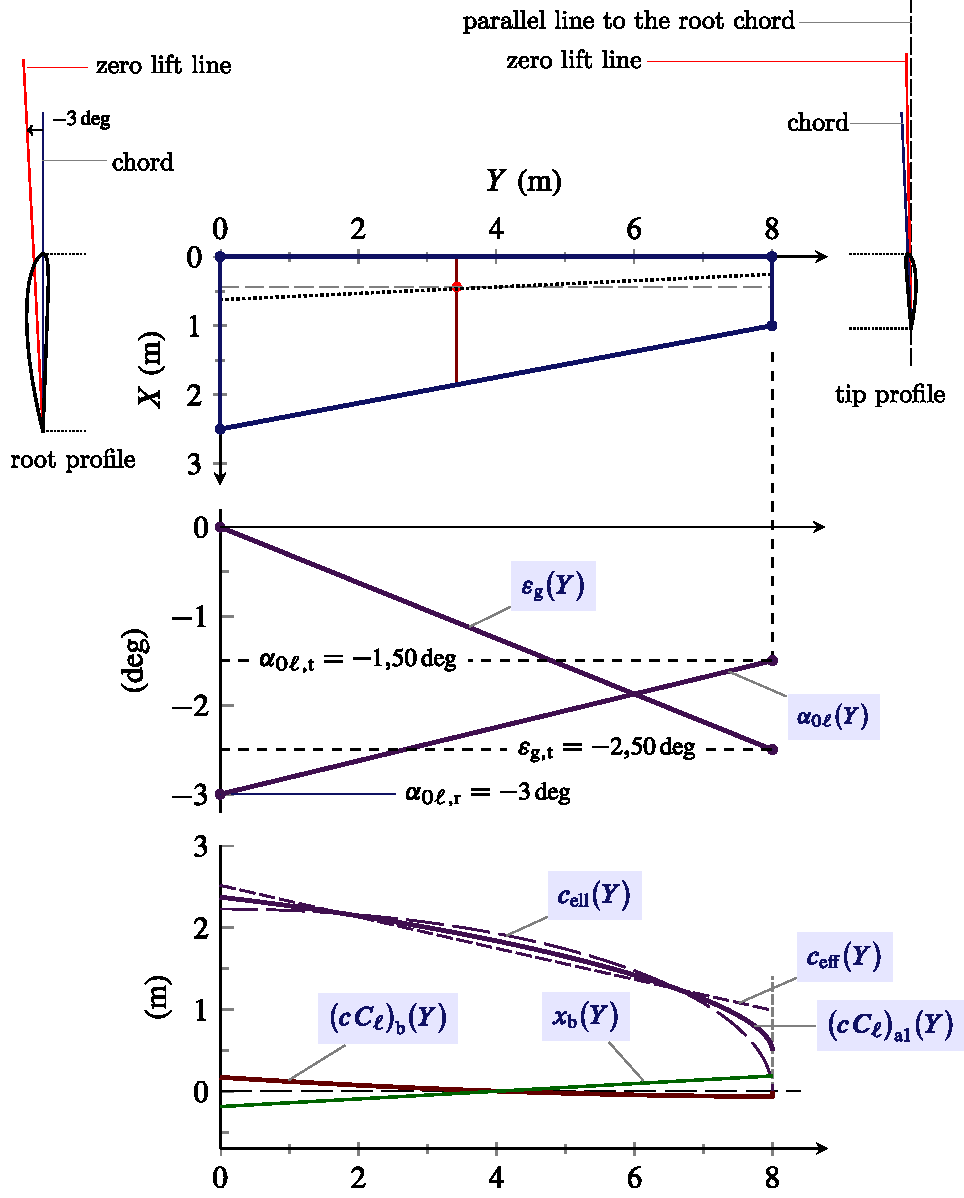
\includegraphics[width=0.90\textwidth]{Chapter_2/pitching_moment/wing_Cmac_1_loading_drawing.pdf}%
    }% end-of-makebox
    \vspace{0.3cm}
  }% #2: the image file included by \includegraphics
  {\finalhyphendemerits=1000
    Wing assigned in the example~\ref{example:Wing:Cmac:A}.
    Law of geometric warping $\epsilon_\mathrm{g}(y)$ and aerodynamic twisting
       $\alpha_{0\ell}(Y)$.
    Additional loading diagrams $(cC_\ell)_\mathrm{a1}$, 
    of the basic loading $(cC_\ell)_\mathrm{b}$ and  of the arm $x_\mathrm{b}(Y)$.%
  }% #3: the caption text
  {fig:Wing:Cmac:Results:A}%% #4: the label
    \end{document}